\pdfoutput=1
\documentclass[10pt,oneside]{article}
\usepackage{microtype}
\usepackage{tikz}
\usepackage{amssymb, amsmath, mathrsfs, graphicx} % remove unneeded packages 
\usepackage{fancyhdr, lastpage, titlesec}
\usepackage[colorlinks]{hyperref}
\usepackage[margin=1in]{geometry}
\pagestyle{fancy}
%\setlength{\columnsep}{2em}
\fancyhead[LO,RE]{Math 275, A. Smith}
\fancyhead[RO,LE]{Page \thepage\ of \pageref{LastPage}}
\chead{\textbf{Test 1, Linear Systems and Matrices}}
\cfoot{}
\parindent 0em
\newcommand{\A}[1]{%
   \begin{tikzpicture}
     \node[draw,circle,inner sep=1pt] {#1};
   \end{tikzpicture}}
\newcommand{\E}[1]{%
   \begin{tikzpicture}
     \node[draw,rectangle, inner sep=5pt] {#1};
   \end{tikzpicture}}


\newcommand{\blank}[1]{\underline{\hspace{#1}}}
\renewcommand{\labelenumi}{\textbf{\thesection.\arabic{enumi}.}}
\newcommand{\las}{\href{http://uwstout.courses.wisconsin.edu/d2l/shibbolethSSO/wayf.d2l}{Learn@UW-Stout }}
\newcommand{\ww}{\href{https://webwork.uwstout.edu/webwork2}{WeBWorK }}


\titleformat{\section}[runin]
{\large\bfseries}
{Part \thesection.}{0pt}{}
\titlespacing{\section}
{\parindent}{2em}{1em}



\newcommand{\edit}[1]{{\color{orange} {\tt((}#1{\tt))}}}
\begin{document}

\setcounter{section}{-1}

\vspace{3in}
\begin{center}
{\tiny Do NOT write your name on this test.}

\vspace{1in}
{\Huge Author code: \A{\phantom{0}}\A{\phantom{0}}\A{\phantom{0}}\A{\phantom{0}}\A{\phantom{0}}}
\end{center}



\vfill


\section{~Instructions}
\begin{enumerate}
\item This test is in-class on Monday February 13, 2016.  It is intended to take
55 minutes.  You must hand it in after 60 minutes.

\item Calculators and computers are not allowed.
%but is not necessary for full credit.  A clear
%and correct expression for the solution will receive full credit even if
%you do not produce a decimal number.
%  (\textbf{Note!} a number like $\frac{2}{3}$ is
%preferred versus $0.66666666$.  Decimal round-offs with a calculator
%\textbf{will} lead to completely incorrect answers in row-reduction!)

\item Network-connected devices are not allowed. 

%\item Notes and Textbooks are not allowed.
\item You may use one sheet (8.5$\times$11 US Letter, both sides) of notes. 

\item Space provided should be adequate for complete answers with average
handwriting.  But, if you don't have enough space, feel free to write on the
blank pages.  If you do so, please mark the work clearly, so that the grader can find it without difficulty.

\item Other students may be taking the test at other times.  For the sake of
fairness and integrity, do \textbf{not} communicate with other students about
the contents, difficulty, emphasis, or style of the test.  This embargo is in
place until 5pm on Tuesday Feb 14.

\item This test is worth 20 points, which are evenly-distributed across the
pages.

\item For full credit, show your thought process clearly, but also
keep your explanations as concise as possible.  A number in a box with no
explanation yields no credit!

\item Don't worry too much about simplification.  In some cases,
``$4\cdot3\cdot2\cdot1$''
is more clear than ``$24$'' if it helps the reader follow your work.

\item Within each Part, symbols (like $A$ or $f(x)$) mean the same thing.  However,
unless explicitly noted, symbols mean something completely different
in different Parts.

\item Be polite to your referee --- Make your work clear and easy to
understand.
\end{enumerate}



\begin{center}
{\Large
\begin{tabular}{r|r|r|r||r}
Page 2 & Page 3 & Page 4 & Page 5 & TOTAL\\\hline
     & \\ 
 /5  & /5 & /5 & /5 & /20 
\end{tabular}}\\
\end{center}
\hfill{\Huge Referee: \E{\phantom{0}}\E{\phantom{0}}\E{\phantom{0}}\E{\phantom{0}}}


\newpage
\section{ }
Perform row-reduction to solve this system.  (Hint!  The final solution is $(x,y,z) =
(4,6,8)$.  You still need to do the work, though.)
\[
\begin{cases}
4x + 24y +0z = 160\\
13x + 47y - 6z = 286\\
12x + 78y + 1z = 524\\
\end{cases}\]


\newpage
\section{ }
Write down all of the $3 \times 4$ reduced row-echelon form matrices that have
rank 2.\\
(Use $\ast$ to indicate entries that could be any number.)

\vspace{2in}
\section{ }
Suppose that $A$ is a $4 \times 4$ matrix for which the following procedure
yields $I$.  First, swap $\rho_2$ and $\rho_4$.  Second, replace
$\rho_1$ with $\rho_1 + 5\rho_3$.  Third, multiply $\rho_3$ by 6, and divide
$\rho_1$ by 5.  Finally, replace $\rho_4$ with $\rho_4 - 3 \rho_1$.
Recall that these row-operations can be un-done in the correct order, to change $I$ back to $A$.
Find the matrix $A$.

\newpage
\section{ }
Suppose that $A$ is a $3 \times 3$ matrix and that $E_1, E_2, \ldots, E_k$ are
elementary matrices such that 
\[ 
 E_k \cdots E_2 E_1 A =  R = \begin{pmatrix}
1 & 0 & \frac15\\
0 & 1 & -3\\
0 & 0 & 0
\end{pmatrix},\quad\text{and}\quad
E_k \cdots E_2 E_1 
=
 \begin{pmatrix}
4 & 2 & 8\\
8 & 1 & 3\\
0 & 1 & 1
\end{pmatrix}.
\]
\begin{enumerate}
\item
Find the solution of the system $A\vec{x}=\vec{0}$ in parametric form.

\vspace{2in}

\item 
Write the solution to the inhomogeneous system 
\[ A \begin{pmatrix}
x_1 \\ x_2 \\ x_3
\end{pmatrix} = \begin{pmatrix}\frac12 \\ -3 \\ 3\end{pmatrix},\]
or explain precisely why no solution exists.

\vspace{2in}

\item 
Write the solution to the inhomogeneous system 
\[ A \begin{pmatrix}
x_1 \\ x_2 \\ x_3
\end{pmatrix} =  \begin{pmatrix}1 \\ 39 \\ -9\end{pmatrix},\]
or explain precisely why no solution exists.

\end{enumerate}

\newpage
\section{ }
The following pictures show two lines, corresponding to a system of two linear equations
in two variables, $[A|b]$.
For each picture, answer these questions:
\begin{itemize}
\item Is the system homogeneous or inhomogeneous?
\item How many solutions does the system have?
\item What is the rank of the $2 \times 2$ matrix $A$?
\item What is the rank of the $2 \times 3$ augmented matrix $[A|b]$?
\end{itemize} 

\begin{enumerate}

\item
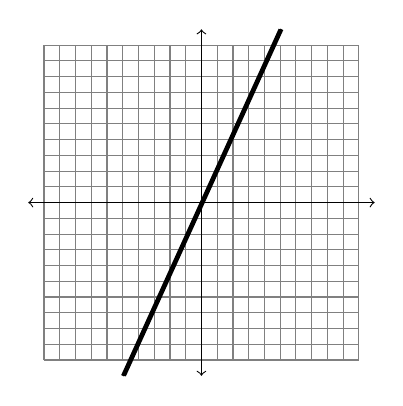
\begin{tikzpicture}[scale=0.2]
\draw[step=1cm, gray, thin] (-10,-10) grid (10,10);
\draw[<->] (-11,0) -- (0,0) --  (11,0);
\draw[<->] (0,-11) -- (0,0) --  (0,11);
\draw[black, very thick] (-5,-11) -- (5,11);
\draw[black, very thick] (-4.9,-11) -- (5.1,11);
\end{tikzpicture} 

\item
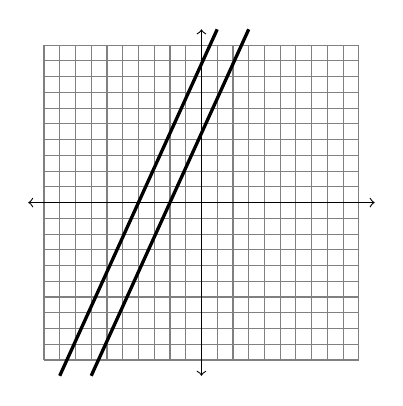
\begin{tikzpicture}[scale=0.2]
\draw[step=1cm, gray, thin] (-10,-10) grid (10,10);
\draw[<->] (-11,0) -- (0,0) --  (11,0);
\draw[<->] (0,-11) -- (0,0) --  (0,11);
\draw[black, very thick] (-7,-11) -- (3,11);
\draw[black, very thick] (-9,-11) -- (1,11);
\end{tikzpicture} 

\item
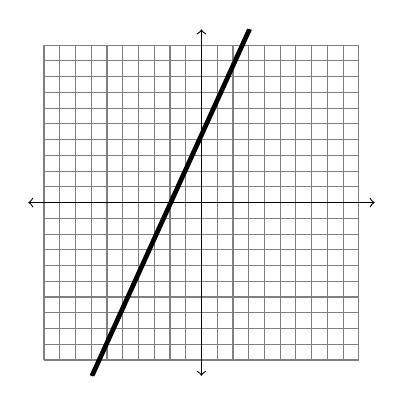
\begin{tikzpicture}[scale=0.2]
\draw[step=1cm, gray, thin] (-10,-10) grid (10,10);
\draw[<->] (-11,0) -- (0,0) --  (11,0);
\draw[<->] (0,-11) -- (0,0) --  (0,11);
\draw[black, very thick] (-7,-11) -- (3,11);
\draw[black, very thick] (-6.9,-11) -- (3.1,11);
\end{tikzpicture} 

\item
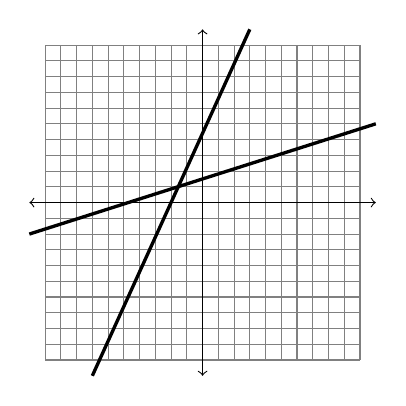
\begin{tikzpicture}[scale=0.2]
\draw[step=1cm, gray, thin] (-10,-10) grid (10,10);
\draw[<->] (-11,0) -- (0,0) --  (11,0);
\draw[<->] (0,-11) -- (0,0) --  (0,11);
\draw[black, very thick] (-7,-11) -- (3,11);
\draw[black, very thick] (-11,-2) -- (11,5);
\end{tikzpicture} 


\end{enumerate}


%%%% END %%%%
\end{document}
